\section{Model}
\label{Sec: model}
\subsection{Uncertainty for model}

In the nominal model, we assume that $D_{s}^{+}$ decays into $X(1385)
e^{+} \nu_{e}$ and $X(1385)$ decays into $p\bar{p}$ pairs.

To estimate the uncertainty caused by model, we compare the
efficiencies for the nominal model and $(p\bar{p})_{S}$-wave model as shown in Tab.
\ref{Tab: model err}. So we set the uncertainty associated with model
at $18\%$.  
\begin{table}[bthp]
    \caption{The efficiencies for the nominal and $(p\bar{p})_{S}$-wave model,
    respectively.}        
    \label{Tab: model err}
    \begin{center}
    \begin{tabular}{lc}
        \hline \hline
        model    &    $ \epsilon $     \\ \hline
        $D_{s}^{+} \rightarrow X(p\bar{p}) e^{+} \nu_{e}$ &
        $(16.7 \pm 0.1 )$ \%      \\ 
        $D_{s}^{+} \rightarrow (p \bar{p})_{S} e^{+} \nu_{e}$    &
        $(20.4 \pm 0.1 )$ \%          \\ 
        \hline \hline
    \end{tabular}
    \end{center}
\end{table}

The big uncertainty associated with the model is caused mainly by the
difference of distribution of proton momentum of each model, since that
the PID efficiency of the proton reduces shapely at low momentum. The
distribution of proton momentum is shown in Fig.  \ref{Fig:
distribution of momentum of proton}.
And the comparison of proton momenta distribution is shown in Fig. \ref{fig:PofPrTruth.eps}.

\begin{figure}[htbp]
    \centering
    \begin{overpic}[ width = 6 cm]{section/append/fig/momentum_signalMC_x1835.eps}
        \put(65,75){$X(p\bar{p})$}
    \end{overpic}
    \begin{overpic}[ width = 6 cm]{section/append/fig/momentum_signalMC_PHSP.eps}
        \put(65,75){$(p\bar{p})_{S}$}
    \end{overpic}
    \caption{Proton momentum distribution based on the MC truth
    information. Left: $p\bar{p}$ from $X(p\bar{p})$. Right: $p\bar{p}$
in S-wave.}
    \label{Fig: distribution of momentum of proton}
\end{figure}
\begin{figure}[htbp]
    \begin{center}
    \mbox{
        \begin{overpic}[width = 8 cm]
            {/besfs/groups/jpsi/jpsigroup/user/maxx/4180/PPbarEnu_newPID/Swave/draw/fig/PofPrTruth.eps}
        \put(25,70) { }
        \end{overpic}
    }
    \end{center}
    \caption{The proton momenta distribution of MC truth information.
        The black solid and red solid line denote events for $X(p\bar{p})$ model
and $(p\bar{p})_{S}$-wave model, respectively.}
    \label{fig:PofPrTruth.eps}
\end{figure}


The momenta distribution of electron is difference for two models shown
in Fig. \ref{Fig: compare pele}, same for $MM^{2}$, so the requirement
on the momenta of electron and $MM^{2}$ may also some uncertainty, and
those uncertainties are covered by model item.
\begin{figure}[htbp]
    \centering 
    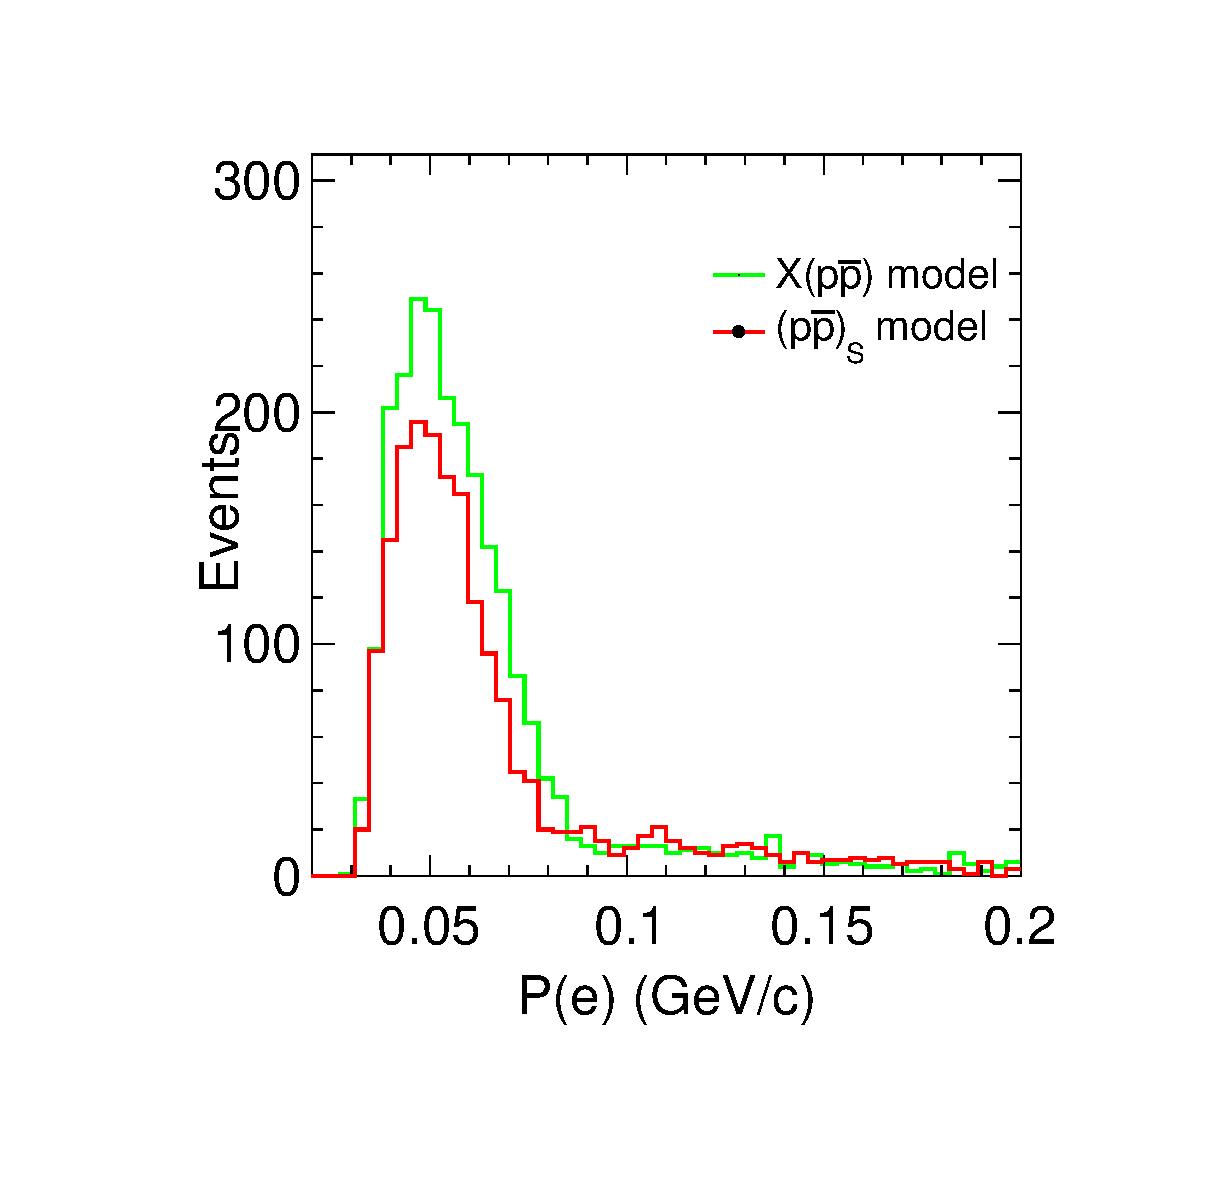
\includegraphics[width = 6cm ]{section/append/fig/momentum_ele_signalMC_PHSP.eps}
    \includegraphics[width = 6cm ]{section/append/fig/MM_signalMC_PHSP.eps}
    \caption{Compare the $MM^{2}$ and electrons' momenta distribution
    between $X(p\bar{p})$ model and $(p\bar{p})_{S}$-wave model.}
    \label{Fig: compare pele}
\end{figure}

The transverse momenta distributions of electron and proton for signal
MC sample are shown in Fig. \ref{Fig: transverse momenta}.
\begin{figure}[htbp]  %pt of electron and proton
    \begin{center}
        \mbox{
            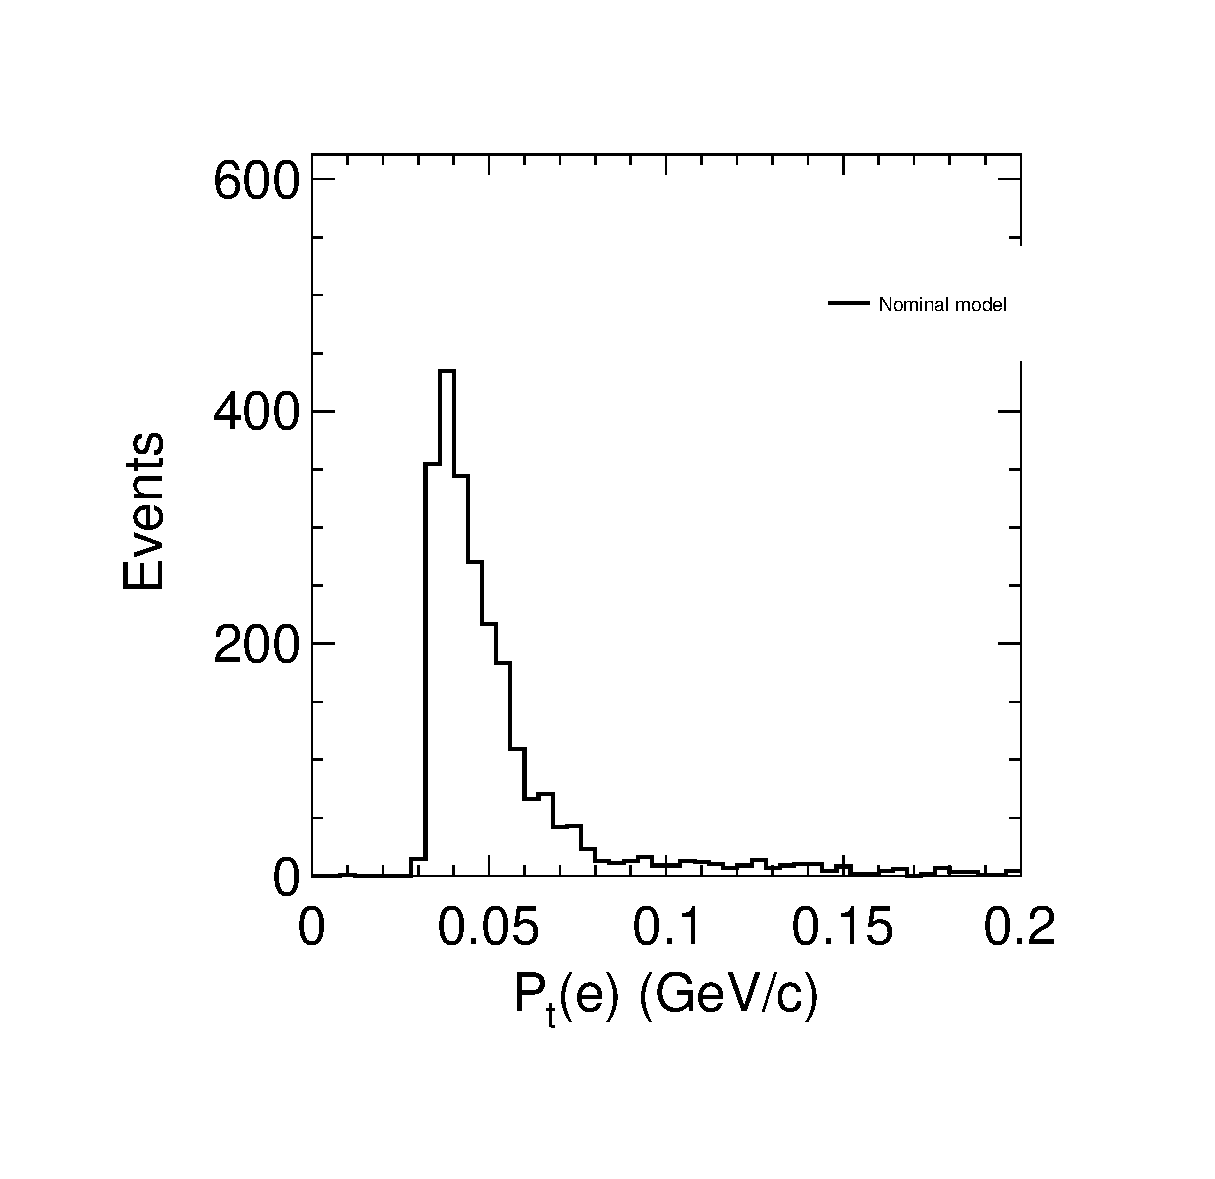
\includegraphics[width = 8 cm]
            {../../signal_model/draw/fig/PtEle.eps}
            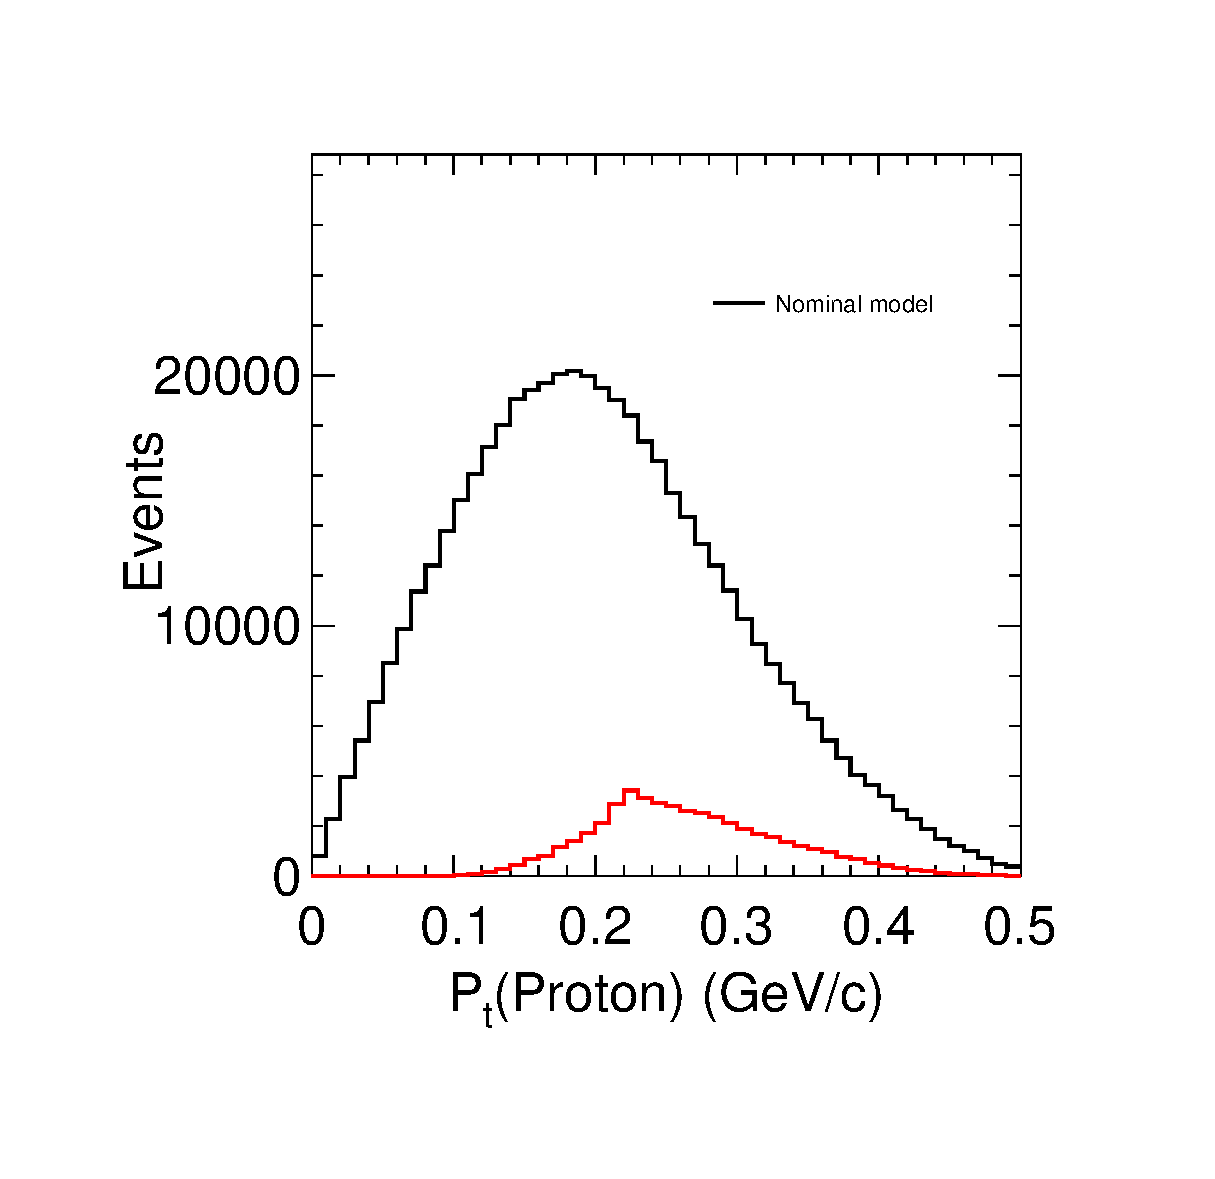
\includegraphics[width = 8 cm]
            {../../signal_model/draw/fig/PtPr.eps}
        }
    \end{center}
    \caption{The transverse momenta distributions. The black line shows
        the transverse momenta distributions for electron and proton 
    with only tracking requirement.}
    \label{Fig: transverse momenta}
\end{figure}

The truth transverse momenta distributions of electron and proton for
signal MC sample are shown in Fig. \ref{fig: TruPtEle}, without any
event selection requirement.

The right plot of \ref{Fig: transverse momenta} from that of \ref{fig:
TruPtEle}, because the former is based on the reconstructed information
after tracking requirement while the later based on truth information
without any requirement.


\begin{figure}[htbp] % truth information for electron and proton
    \begin{center}
    \mbox{
        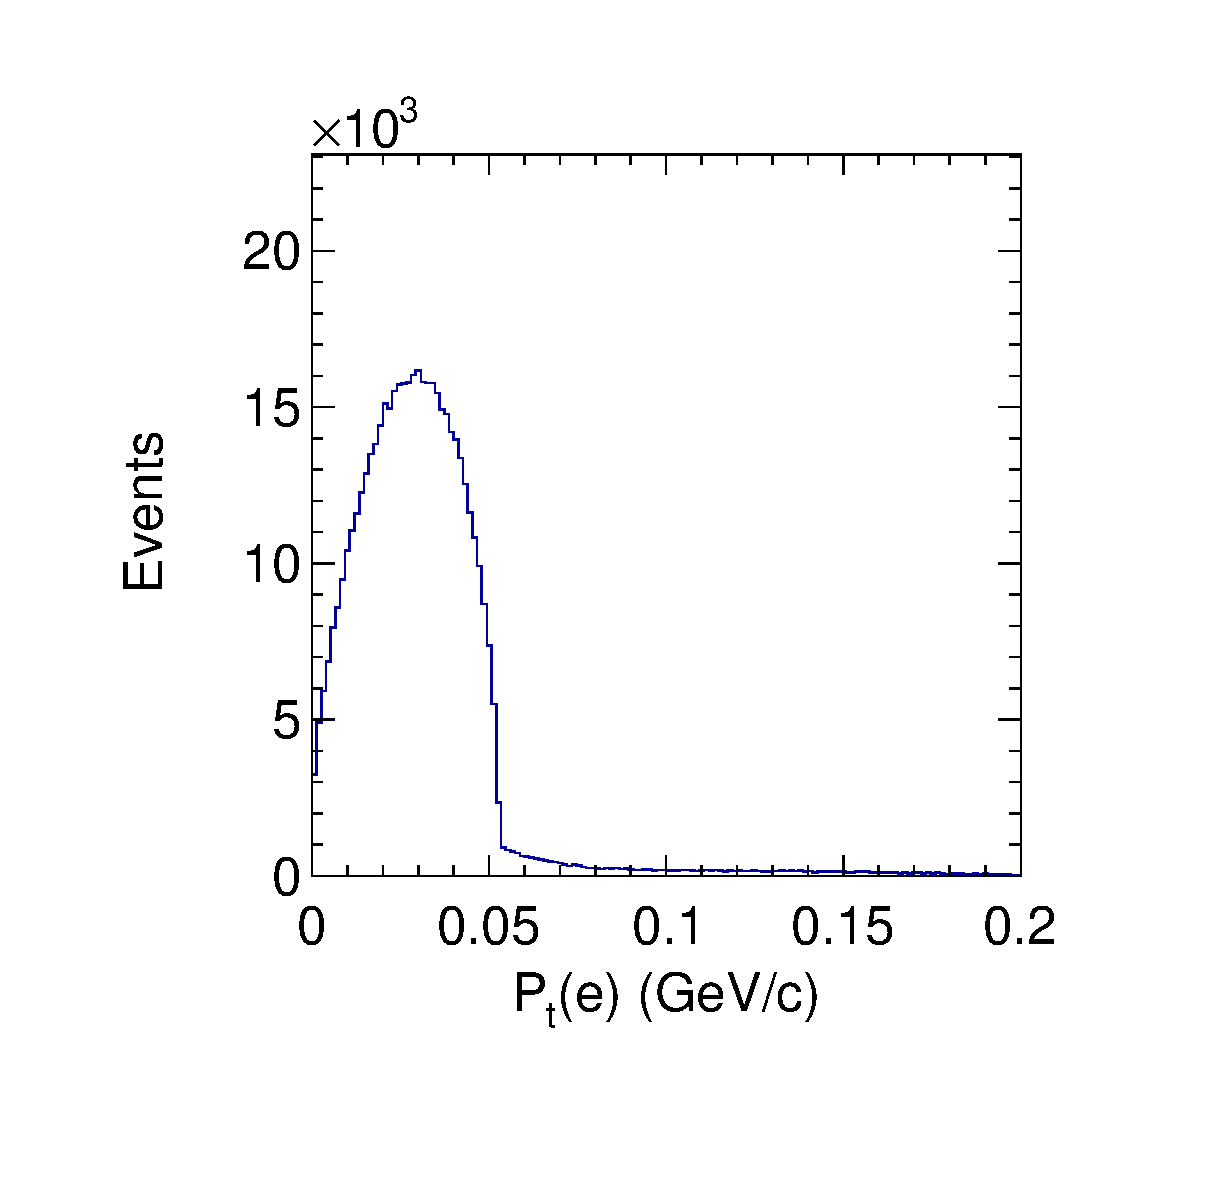
\includegraphics[width = 8 cm]
        {../../signal_model/draw/fig/TruPtEle.eps}
        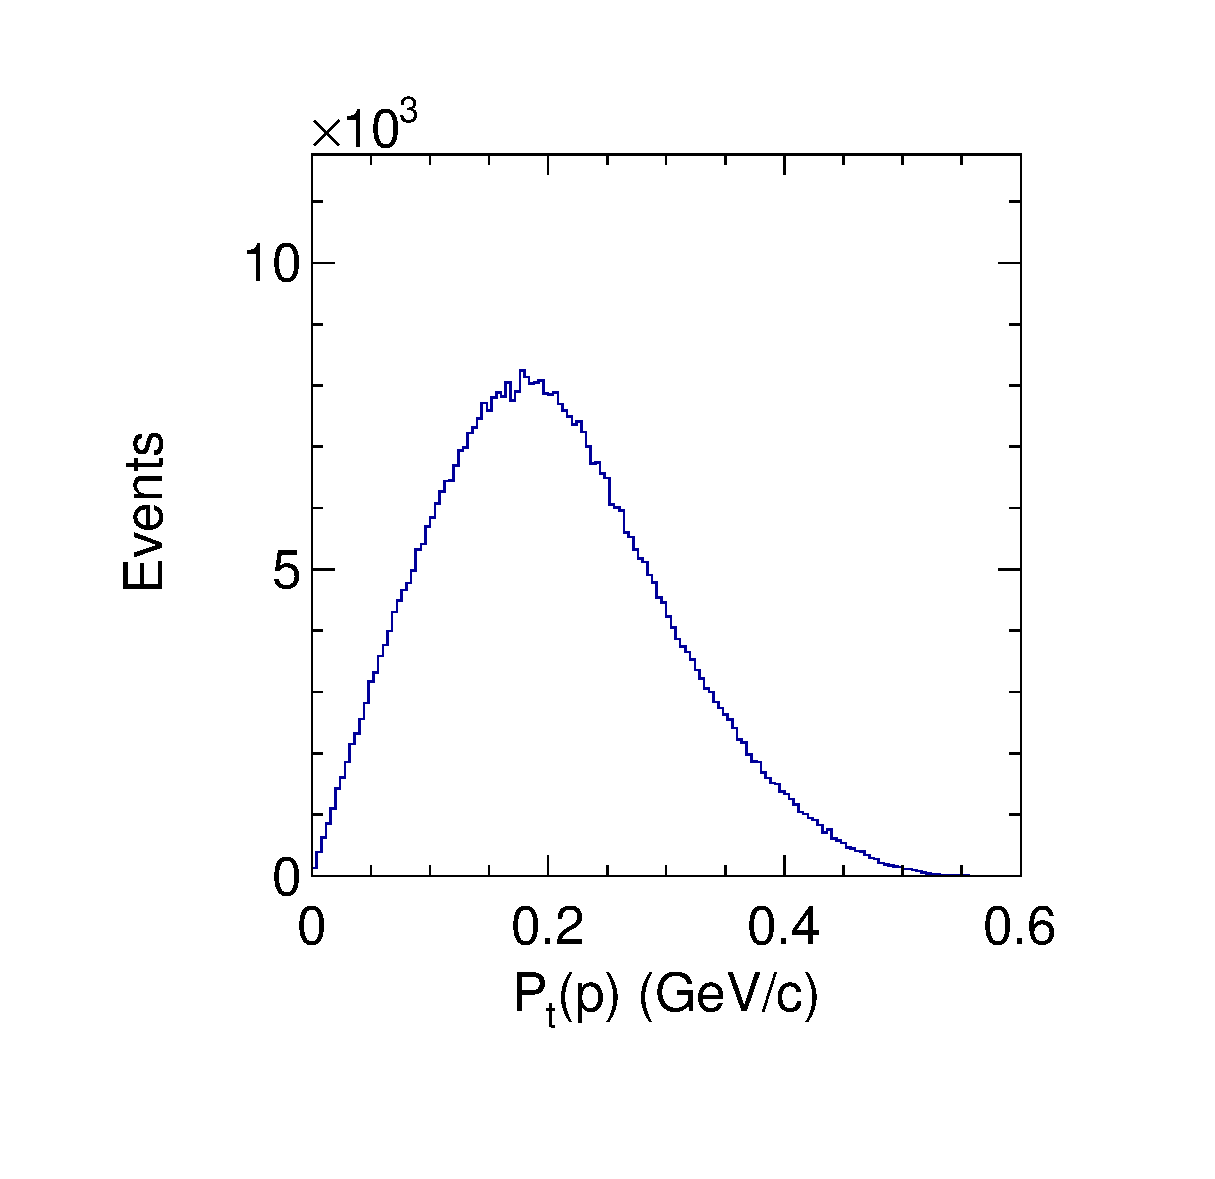
\includegraphics[width = 8 cm]
        {../../signal_model/draw/fig/TruPtPr.eps}
    }
    \end{center}
    \caption{The MC truth information.}
    \label{fig: TruPtEle}
\end{figure}

\subsection*{Efficiency}
Due to the low momenta of proton, the efficiency is very sensitive to
the $M(p\bar{p})$ distribution. The Fig. \ref{fig: eff_mpp} shows the
efficiency line. We can see the efficiency vary from 10\% to 50\%.

The line shape of $X(p\bar{p})$ is shown in Fig. \ref{fig: XShape}.
\begin{figure}[htbp]
    \begin{center}
    \mbox{
        \includegraphics[width = 8cm]{../../signal_MC/draw/fig/eff_mPP.eps}
    }
    \end{center}
    \caption{The $\epsilon$ is the DT efficiency over ST efficiency.}
    \label{fig: eff_mpp}
\end{figure}

\begin{figure}[htbp]
    \begin{center}
    \mbox{
        \includegraphics[width = 8cm]{../../signal_MC/draw/fig/XShape.eps}
    }
    \end{center}
    \caption{The line shape off $X(p\bar{p})$, which is described by
    relativistic Breit-Wigner function.}
    \label{fig: XShape}
\end{figure}

\subsection{Uncertainty for $X(p\bar{p})$}
\label{uncertainties for Xpp}
The width of $X(p\bar{p})$ is vary from 10 MeV to 80 MeV, and
the efficiencies are obtained by re-weighting binned efficiency.
From Fig. \ref{fig: vary Mass and width}, we can see the efficiency
vary from 16\% to 17\%, 
so the uncertainty associated with the width as 1\%.

Similarly, vary the mass of $X(p\bar{p})$ from 1.80 GeV to 1.85 GeV,
the efficiency change in range 2\%. So set 2\% as the uncertainty
associated with the mass.

\begin{figure}[htbp]
    \begin{center}
    \mbox{
        \includegraphics[width = 8
        cm]{../../signal_MC/reweight/fig/effLine.eps}
        \includegraphics[width = 8
        cm]{../../signal_MC/reweight/fig/varyM.eps}
    }
    \end{center}
    \caption{Vary the width and mass of $X(p\bar{p})$.}
    \label{fig: vary Mass and width}
\end{figure}

